%%% Please, do not change any of the following parameters.
\documentclass[10pt,journal,compsoc,twoside]{IEEEtran}
\usepackage{cite}
\usepackage{graphicx}
\usepackage{amsmath}
%\interdisplaylinepenalty=2500
\usepackage{algorithmic}
\usepackage{array}
\usepackage[caption=false,font=footnotesize]{subfig}
\usepackage{url}
\usepackage{lipsum}
\usepackage{hyperref}
\usepackage{pgfplotstable}
\usepackage{pdflscape}
\usepgfplotslibrary{units}
\hypersetup{pdfborder = 0 0 0}
\PassOptionsToPackage{hyphens}{url}\usepackage{hyperref}


\pgfplotstableset{
	begin table=\begin{longtable}, % -------- CF
		end table=\end{longtable},
	every head row/.style={
		%before row=\caption{X-Powered-By header}\\\toprule, after row=\bottomrule \endhead,% --------- CF
		% as in the previous example, this patches the first row:
		before row={\hline},
		after row=\hline,
	},
	every last row/.style={% ------------ CF
		after row=\hline,
	},
	every even row/.style={
		before row={\rowcolor[gray]{0.92}}},
}

\pgfplotsset{compat=newest} 

\pgfplotsset{
	select row/.style={
		x filter/.code={\ifnum\coordindex=#1\else\def\pgfmathresult{}\fi}
	},
	discard if/.style 2 args={
		x filter/.code={
			\edef\tempa{\thisrow{#1}}
			\edef\tempb{#2}
			\ifx\tempa\tempb
			\def\pgfmathresult{inf}
			\fi
		}
	},
	discard if not/.style 2 args={
		x filter/.code={
			\edef\tempa{\thisrow{#1}}
			\edef\tempb{#2}
			\ifx\tempa\tempb
			\else
			\def\pgfmathresult{inf}
			\fi
		}
	}
}


\graphicspath{ {figures/} } %%% put all images file into "figures/" subdirectory

\begin{document}

\title{Optimization of screen-space directional occlusion algorithms}

\author{Dominik Szajerman, Marcin Wawrzonowski%
\IEEEcompsocitemizethanks{\IEEEcompsocthanksitem Lodz University of Technology, {\L}{\'o}d{\'z}, Poland, \hfil\break 207612@edu.p.lodz.pl}}


% The paper headers
\markboth{Computer Game Innovations, 2017}%
{Marcin Wawrzonowski \MakeLowercase{\textit{et al.}}: Optimization of screen-space directional occlusion algorithms}

\IEEEtitleabstractindextext{%
\begin{abstract}
%%% 100 words
Developers of video games and simulations from the day one have been trying to improve
visuals of their products. One of the methods to simulate global illumination without a lot of processing is Screen-Space Ambient Occlusion. Many implementations of this technique were
created, though few take into account direction and colour of the incoming light. An exception is a technique named SSDO –- Screen-Space Directional Occlusion. Unfortunately,
it suffers from the same drawbacks as its less realistic cousins, such as noise and banding
while also remaining moderately expensive for computation. The main purpose of this paper
is to optimize basic SSDO method using technique called Statistical Volumetric Obscurance,
enhancing its performance while retaining plausible visual effect.
\end{abstract}

\begin{IEEEkeywords}
computer games, computer graphics, rendering, global illumination, screen-space, ambient occlusion, directional occlusion, volumetric obscurance
\end{IEEEkeywords}}

\maketitle
\IEEEdisplaynontitleabstractindextext
\IEEEpeerreviewmaketitle
\IEEEraisesectionheading{
\section{Introduction}\label{t:introduction}
}
Since the beginning of the video games industry, developers struggled to achieve the best looking and most realistic graphics. Possibly the most important factor in this matter is illumination of the virtual scene. Methods like ray-tracing or radiosity, which are very accurate and produce realistic results are still too computationally expensive to be used in real-time applications. Because of that, many techniques were created to approximate them while achieving good performance as well. Among these methods, one of the most important and popular one is SSAO -- Screen-space Ambient Occlusion. It introduces additional darkening in places, where it would be difficult for light to reach. Many techniques of generating SSAO were created, but most of them suffer from similar problems, such as undersampling, noises, banding and other visual artefacts. It is not related to light direction or colour, as it usually appears as a~separate postprocess. An improvement to this situation is a technique named Screen-Space Directional Occlusion. Its main feature is combining computations with light calculations, allowing to take into account colour and direction of light. A way to produce an additional one bounce of light was also presented, allowing to approximate global illumination model more closely. While SSDO can be easily computed in real-time, it is still moderately expensive for performance. A main purpose of this paper is to optimize the SSDO technique while maintaining its visual features and keeping, or insignificantly reducing, their quality. It was achieved by employing an algorithm named Statistical Volumetric Obscurance (StatVO). Its main characteristic is a~replacement of traditional SSAO sampling with a statistical model, based on precomputing an average value of depth in the neighbourhood of a pixel. In this paper, all aforementioned techniques are discussed, all their key equations and algorithms are presented. Then, the proposed solutions are described, which consist of two techniques based on StatVO model. The most important difference between them is the average input data generation process. After this, test methods and their results are presented. Tests are conducted between the original SSDO technique and two novel ones. In the last chapter, test results are discussed, methods are compared in regard to the performance and visual quality. A ways to enhance them further are also presented.

\section{Related work}\label{t:related}

	\subsection{Screen-space Ambient Occlusion}\label{t:related:ssao}
	
	A basic ambient occlusion algorithm uses local geometry around a given point on an object's mesh as the input data. For every such point, a set of random, but evenly distributed rays is generated. This distribution can have shape of a~sphere or a hemisphere, if the surface normal vector is taken into account \cite{ao}. Whole process is described in the figure \ref{fig:2_A} below.
	
	\begin{figure}[ht] %%% example figure (PNG format for bitmaps and PDF format for vector images are preferred)
		\centering
		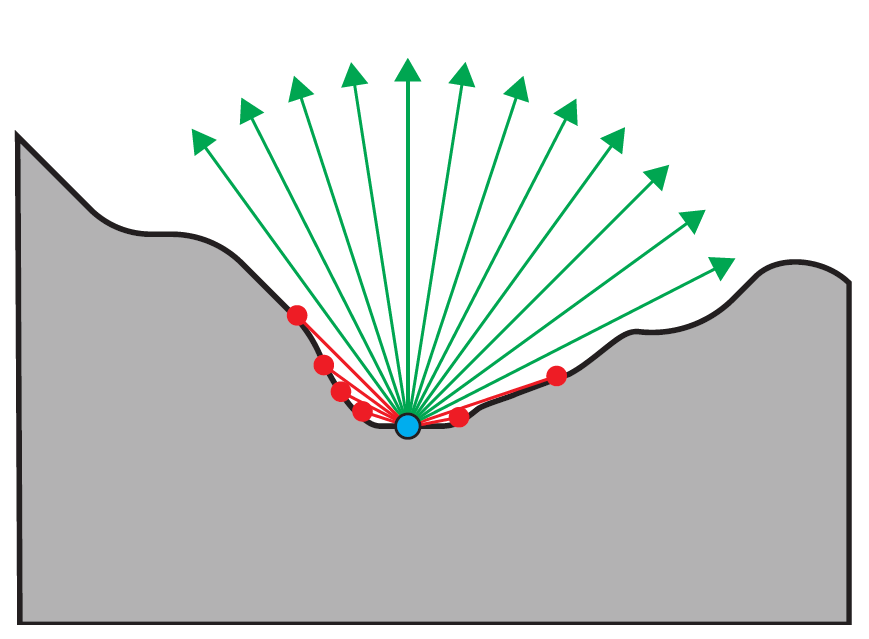
\includegraphics[width=0.4\textwidth]{fig_2_A.png}
		\caption{Essence of the ambient occlusion method \cite{statvo}.}
		\label{fig:2_A}
	\end{figure}

	An ambient occlusion for a given point is described by a ratio of the number of outgoing rays which hit neighbouring geometry to the number of all rays. It is formally defined in \cite{sloan} as:
	
	\begin{equation}
	\mathit{AO}(\mathbf{x}, \vec{n}) = \frac{1}{\pi}\int_{\Omega}^{}\rho(\mathit{d}(\mathbf{x}, \vec{\omega},))\vec{n}\cdot \vec{\omega}d\vec{\omega}\ ,
	\end{equation}
	
	where \(\mathbf{x}\) stands for a position in the scene, \(\Omega\) represents sampling directions and \(d\) is the distance from the ray's first hit. \(\rho\) is usually an user-defined \textit{falloff} function, which relates \(d\) with the final occlusion effect. In most cases it is linear or quadratic function. Presented method is still too costly to be applied in real-time graphics. To solve this problem, a screen-space approach was introduced \cite{crytek}. Instead performing calculations on the geometry, it uses rendered frame's depth buffer, with an optional normal vector buffer. As a replacement for the aforementioned ray tracing, many techniques were invented by the developers, including point sampling, line sampling or horizon-based sampling \cite{statvo}. Similarly, amount of occlusion in the given pixel equals a ratio of the number of ``occluded'' samples (i.e. ``behind'' the depth buffer, with a higher depth that can be directly sampled from it) to the number of all samples. A convenient falloff function is also applied. SSAO can generate very plausible approximation of the ambient light distribution, but suffers from undersampling and noise, because it is a low-frequency effect. A number of samples is usually low to avoid a significant performance drop. In most cases additional blurring is needed to account for these artefacts.
	
	\subsection{Statistical Volumetric Obscurance}\label{t:related:statvo}
	
	This technique (StatVO) bases on a similar assumption as the SSAO does, i.e. the occlusion in each pixel is related to the amount of geometry around it. The difference is that StatVO does not achieve it through sampling. Instead it builds a statistical model based on an average depth. It can be seen in figure \ref{fig:2_B}.
	
	\begin{figure}[ht]
		\centering
		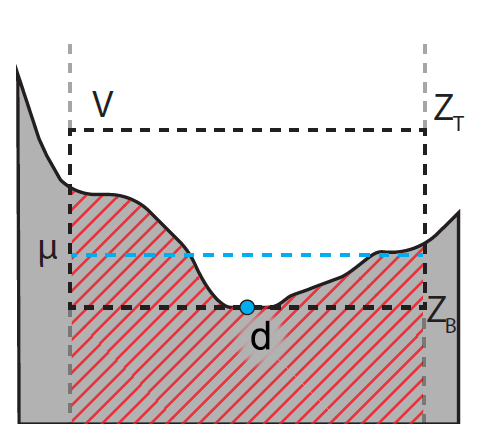
\includegraphics[width=0.35\textwidth]{fig_2_B.png}
		\caption{Essence of the StatVO method \cite{statvo}.}
		\label{fig:2_B}
	\end{figure}

	 A sample box is build around processed point, instead of a sample hemisphere. The authors of \cite{statvo} assume that the bigger is the difference between \(\mu\) and \(d\), the more occlusion occurs in each pixel. This is computed in relation to the \(Z_{T}\) and \(Z_{B}\) parameters and can be seen in equation (2).
	 
	 \begin{equation}
	 \mathit{StatVO}(\mathbf{x}) = \psi(\frac{z_{B}(\mathbf{x}) - \mu(\mathbf{x})}{z_{B}(\mathbf{x}) - z_{T}(\mathbf{x})})\ .
	 \end{equation}
	 
	 Function \(\psi\) is a falloff function. It clamps negative values to 0, behaves linearly in the compartment of [0, 1] and drops down to 0 beyond it. The last behaviour simulates samples falling outside the sampling area in the classic AO approach. As it will be shown in section \ref{t:tests}, thanks to the averaging, StatVO results in a very smooth, noise-free effect, requiring no blurring in the process. It also lowers number of samples in the pixel shader, effectively boosting the performance. Regardless of this, StatVO also possess a~very serious drawback. Because of the statistical approach and computing an average depth value, whole process does not take into account depth discontinuities around rendered objects. It generates unwanted dark halos it such places and special steps must be taken in order to avoid this artefact. One such approach, described in \cite{statvo} is to split depth buffer into separate layers, adaptively to the local geometry. Borders of the layers are created around depth discontinuities. Second approach, involving usage of depth buffer's mip maps was described in section \ref{t:solutions:c}.
	
	\subsection{Summed Area Table}\label{t:related:sat}
	
	A key element in the StatVO technique is fast and error-free generation of the averaged depth buffer. A data structure named Summed Area Table (SAT) was chosen for this purpose by the authors of \cite{statvo}. SAT is a two-dimensional array, where each element corresponds to the sum of the elements above and to the left of him. It is presented in the figure \ref{fig:2_D}.
	
	\begin{figure}[ht]
		\centering
		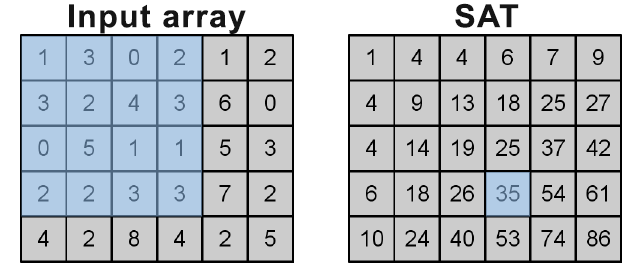
\includegraphics[width=0.4\textwidth]{fig_2_D.png}
		\caption{SAT example \cite{sat}.}
		\label{fig:2_D}
	\end{figure}

	Value of each cell (\(x\), \(y\)) in SAT is described by equation:
	
	\begin{equation}
	\mathit{SAT}(x, y) = \sum_{x}^{i=1}\sum_{y}^{j=1}\mathit{Input}(i, j)\ ,
	\end{equation}
	
	where maximum values of \(x\) and \(y\) are respectively width and height of the input array. The most important characteristic of sum tables is the fact that finding an average value of any rectangular filter requires sampling only four values. This makes computation time independent of filter size, it equals \(O(1)\). Whole process is described by following equation:
	
	\begin{equation}
	\overline{x} = \frac{x_{A} - x_{B} - x_{C} + x_{D}}{A}\ ,
	\end{equation}
	
	where \(x_{n}\) is a SAT value in the corner of averaged area, counting clockwise and starting from the lower right corner. \(A\) stands for the area of the filter.
	
	\subsection{Screen-space Directional Occlusion}\label{t:related:ssdo}
	
	This technique is an improvement of SSAO, taking account of the direction and colour of incoming light. It also computes one bounce of indirect light, entailing final effect closer to the one generated by global illumination algorithms. Because SSDO uses the same samples to compute both parts of the process, it's similar to the original SSAO in the terms of performance. Authors of \cite{ssdo} remove decoupling between lighting and occlusion computation. They propose the following equation:
	
	\begin{equation}
	L_{dir}(\mathbf{P}) = \sum_{i=1}^{N}\frac{\rho}{\pi}L_{in}(\omega_{i})V(\omega_{i})\cos\theta_{i}\Delta\omega\ .
	\end{equation}
	
	For every pixel in view position \(\mathbf{P}\) direct illumination is computed from \(N\) sampling directions, distributed over a~hemisphere. Each sample calculates a product of incoming light intensity \(L_{in}\), visibility \(V\) and a BRDF function \(\frac{\rho}{\pi}\). A key difference between SSAO and SSDO is classification of the samples, depending on the fact, whether they are ``below'' geometry or ``above''. A depth buffer and depth values of samples are used to compute this factor. Instead of calculating a ratio between occluding samples and all samples to create darkening effect, an illumination is calculated from the ``above'' directions, each classified as ``visible''. The more geometry occurs around sampling point, the less samples are categorized as such, less illumination is computed and the darkening increases, but effect is strictly coupled with light colour and direction. Whole process can be seen in the left part of the figure \ref{fig:2_H}.
	
	\begin{figure}[ht]
		\centering
		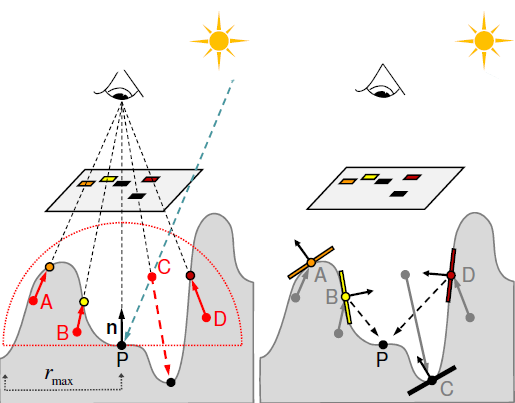
\includegraphics[width=0.4\textwidth]{fig_2_H.png}
		\caption{Essence of the SSDO technique \cite{ssdo}. Left section describes direct illumination, while right shows indirect one.}
		\label{fig:2_H}
	\end{figure}

	In the second pass, SSDO calculates one bounce of indirect light. As for the input data, samples which appear ``below'' the depth buffer are classified as ``not visible'' and used. They are back-projected to the image, then colour and normal buffers are sampled, resulting in acquiring all necessary information about outgoing light. It can be seen in the right part of the figure \ref{fig:2_H}. Indirect illumination is computed according to the equation:
	
	\begin{equation}
	L_{ind}(\mathbf{P}) = \sum_{i=1}^{N}\frac{\rho}{\pi}L_{pixel}(1 - V(\omega_{i}))\frac{A_{s}\cos\theta_{s_{i}}\cos\theta_{r_{i}}}{d_{i}^2} \ ,
	\end{equation}
	
	where \(d_{i}\) is the distance between occluder and \(\mathbf{P}\), \(\cos\theta_{s_{i}}\) and \(\cos\theta_{r_{i}}\) correspond to respectively angles between source and receiver's normal vectors and direction of the incoming light. A value of \(A_{s}\) is used to control the size of the effect. The usage of factor \((1 - V(\omega_{i}))\) assures that indirect illumination won't occur in places where the darkening is present. Usually they appear on the different sides of the object though \cite{ssdo}.
	
\section{Proposed solutions}\label{t:solutions}

The main purpose of this paper was to improve the performance of SSDO algorithm while maintaining similar, or insignificantly worse, visual plausibility. It was done so by employing StatVO instead of traditional sampling method, lowering number of texture look-ups in the pixel shader and removing necessity to blur the final effect. 
For these purposes, two novel SSDO techniques were created, referred to as SSDO-B and SSDO-C. Both are described thoroughly in this section. The original SSDO method discussed in section \ref{t:related:ssdo} will be referred to as SSDO-A.
	
	\subsection{SSDO-B}\label{t:solutions:b}
	
	% SAT computation
	% Adaptive computation
	% Sampling direct
	% Sampling indirect
	
	The first part of this algorithm is SAT data generation process. To acquire average values for each pixel, a summed area table must be generated for two buffers. One consists of normal vectors and depth. The other is a color buffer and is necessary for the indirect light computations. While creating SAT using equation (3) is a trivial process, it may have a serious performance drawback and is completely not suitable for GPU texture data, as it would require transfers between CPU and the GPU. To keep high framerate it is necessary to compute SAT on the GPU itself. In this work, Direct3D 11 compute shaders and Parallel Prefix Sum algorithm \cite{prefix-sum} are used. The method performs computation on each texture row separately and uses a balanced tree concept to determine what each thread does at each step of its traversal. It is divided into two phases, up-sweep and down-sweep. In the first one, tree is traversed from leaves to root, computing partial sums at internal nodes of the tree. After this, a zero is inserted in the root node and down-sweep phase begins. There, each node at the current level passes its own value to its left child, and the sum of its value and the former value of its left child to its right child. In result, a one-dimensional array of sums is created in each row of the texture. To generate SAT itself, an algorithm is launched twice -- vertically and horizontally. To further optimize computations, an offset is introduced when accessing shared memory to prevent bank access conflicts \cite{directcompute}. Also, each thread computes SATs for both input textures at once, reducing the number of compute shader dispatch calls. Summed area tables are generated from second mip level of base textures. It greatly improves performance and has almost no effect on the final result.
	
	As it was explained in section \ref{t:related:statvo}, using one depth buffer for whole rendered scene may result in errors around depth discontinuities. To prevent this, four adaptive layers are created, also with compute shaders. The input data are original parent layers (both textures are processed at once) and their SATs. Having summed area tables, an average depth value can be computed for each input pixel. Then it is assigned to one of the layers, depending on the factor, whether its depth is higher or lower than the average. The idea of this algorithm is that around depth discontinuities, every pixel closer to the camera will have depth value lower than the average and vice versa, therefore they will be assigned to different layers \cite{statvo}. Process is repeated recursively until four input layers are created. The important optimization here is that not every SAT needs to be computed, as for example, child B's SAT value is the difference between corresponding values in parent SAT and child A SAT \cite{statvo}.
	
	Like in original SSDO-A algorithm, directional occlusion computation is divided in two stages -- direct illumination and one bounce of indirect light. To improve performance, both are computed in the same rendering pass. When abandoning sampling method from SSDO-A in favour of statistical model, it is necessary to take into consideration that noticeably different algorithm must be used. In the discussed case, the technique was simplified, but it generates similar effects. Colour and direction of SSDO-A shadowing are strictly dependent of analogous light parameters. This fact was used to limit occlusion generated by StatVO to less illuminated places. A dot product of average normal vector and light direction was used in this matter. Colour of shadowing was related to light colour by multiplication. The latter's vector was normalized before this operation to avoid influence of brightness on the final occlusion effect. Whole process can be described by following equations:
	
	\begin{equation}
	D = saturate(pow(1 - max(\vec{n_{avg}} \cdot \vec{L_{d}}, 0), p))\ ,
	\end{equation}
	
	\begin{equation}
	V = AD(1 - StatVO(\mathbf{x})) \frac{\vec{L_{c}}}{\overline{L_{c}}}\ .
	\end{equation}
	
	\(V\) is the final illumination colour based on SSDO. \(A\)~refers to brightness factor, an external parameter for the algorithm. \(\vec{n_{avg}}\) is an average normal vector for a given pixel, computed using SAT. \(L_{d}\) and \(L_{c}\) are, respectively, light direction and colour.
		
	Indirect bounce of light computing process was also simplified and, basically, it reduces to manipulating averaged colour buffer. It is important to notice that blurred colour, when limited to certain areas, can mimic the effect of SSDO-A light bleeding. The process starts with computing a~difference of pixel colour and the averaged one. In the next step, result is transformed to HSV space, hue component is inverted and whole value is transformed back to RGB space. Because of this, only the colour part which ``bleeds'' is left in the process and it is possible to simply add result to the final value. In the end, indirect light is related with directional factor \(D\), light colour and occlusion by multiplication. Whole process is described by following equation:
	
	\begin{equation}
	I = \rho(c_{\mathbf{x}} - c_{avg})c_{avg}\vec{L_{c}}(1 - D)(1 - StatVO(\mathbf{x}))\ ,
	\end{equation}
	
	where \(\rho\) is a function which transforms to HSV space, flips hue component and restores value back to RGB.
	
	Both stages, indirect and direct, were computed for each of the SAT adaptive layers. Then, results were averaged using SAT of separate index buffer, where in each pixel a~value of 1 is present if a pixel was assigned to corresponding layer and 0 otherwise.
	
	\subsection{SSDO-C}\label{t:solutions:c}
	
	The second proposed solution is a simplification of SSDO-B algorithm. It was created because of the necessity to remove the most computationally heavy part of SSDO-B -- creating adaptive layers and calculating SATs for some of them. It was observed that necessary input data for SSDO-B are simply an averaged normal, depth and color buffers. These can be computed without resorting to SAT, using less expensive methods. It was also important to use algorithm that is aware of depth discontinuities around rendered objects. In the end, a simple Gaussian blur with 5x5 filter was used. Each sample was also weighted by its depth and normal vector differences, cutting out samples which are placed too far away.
	
	Second mip level of base textures is also used as input data. Without depth layering, an error is present where jagged edges of objects in lower-resolution buffers overlap with smooth ones in full-size textures (see part D of figure \ref{fig:4_C} in section \ref{t:tests}). A technique was created to partially solve this issue. It bases on the fact that error results in sharp outlines around objects and they are becoming thicker when lower mip level of input texture is used. Employing a simple difference between depths, these edges can be detected, and occlusion in these places cut out from the final result. 

\section{Test method and results}\label{t:tests}

	Test method consists of two sections. First, the performance of each technique is measured and presented on the chart. The measure units are FPS (Frames Per Second, i.e. how many frames the program is able to compute in the time of one second), \(ms\), what corresponds to time of rendering an one frame of application and \(ms_{R}\) which is the time of computing given technique (i.e. \(ms\) minus all other processing of the program). For reference, an original SSDO technique (SSDO-A) was measured. To show each method's influence on the workload of the application, a situation where no technique is applied was also presented. Measured values were collected in every frame between 10 and 40 second of the program's work time and the final result is an arithmetic average of all of them.
	
	In the second section, visual result of each technique (along with the original one) is displayed. For each method, four screenshots were taken. The ones marked A and B concentrate on showing occlusion effects and C shows indirect lightning. Each category was created with the same position of the camera in scene. Pictures marked with letter D are different for each method and concentrate on presenting errors that can occur for used technique. The coloured rectangles and circles have been placed in the graphics program and serve only as indicators of important elements on images.

	\begin{table}[!ht]
		\caption{The performance of implemented SSDO techniques}
		\label{tab:example}
		\centering
		\begin{tabular}{|c|c|c|c|}
			\hline
			\textit{Method} & \textit{FPS} & \(ms\) & \(ms_{R}\) \\ 
			\hline\hline
			SSDO-A & 793 & 1.26 & 0.91 \\ 
			SSDO-B & 362 & 2.76 & 2.41 \\ 
			SSDO-C & 2130 & 0.46 & 0.12 \\ 
			None & 2880 & 0.34 & 0 \\ 
			\hline
		\end{tabular}
	\end{table}
	
	\pgfplotstableread
	{
		method fps
		SSDO-A 793
		SSDO-B 362
		SSDO-C 2130
		None 2880
	}\loadedtable
	
	\pgfplotstableread[header=false]{
		793 SSDO-A
		362 SSDO-B
		2130 SSDO-C
		2880 None
	}\datatable
	
	\begin{figure}
		\begin{tikzpicture}
		\begin{axis}[
		xbar, bar shift=0pt,
		enlarge y limits=0.2,
		xmin=0,
		xtick={0, 800, 1600, 2400, 3200},
		ytick={0,...,4},
		axis x line*=bottom,
		axis y line*=left,
		yticklabels from table={\datatable}{1},
		xmajorgrids = true,
		bar width=8mm, 
		width=8cm, height=5.5cm, 
		xlabel={FPS},
		ylabel={SSDO technique},
		nodes near coords, nodes near coords align={horizontal},
		]
		
		\pgfplotsinvokeforeach{0,...,4}{
			\addplot table [select row=#1, y expr=#1] {\datatable};
		}
		\end{axis}
		\end{tikzpicture}
		\caption{The performance of implemented SSDO techniques.}
		\label{wykr_7_A}
	\end{figure}

	\begin{figure}[ht]
		\centering
		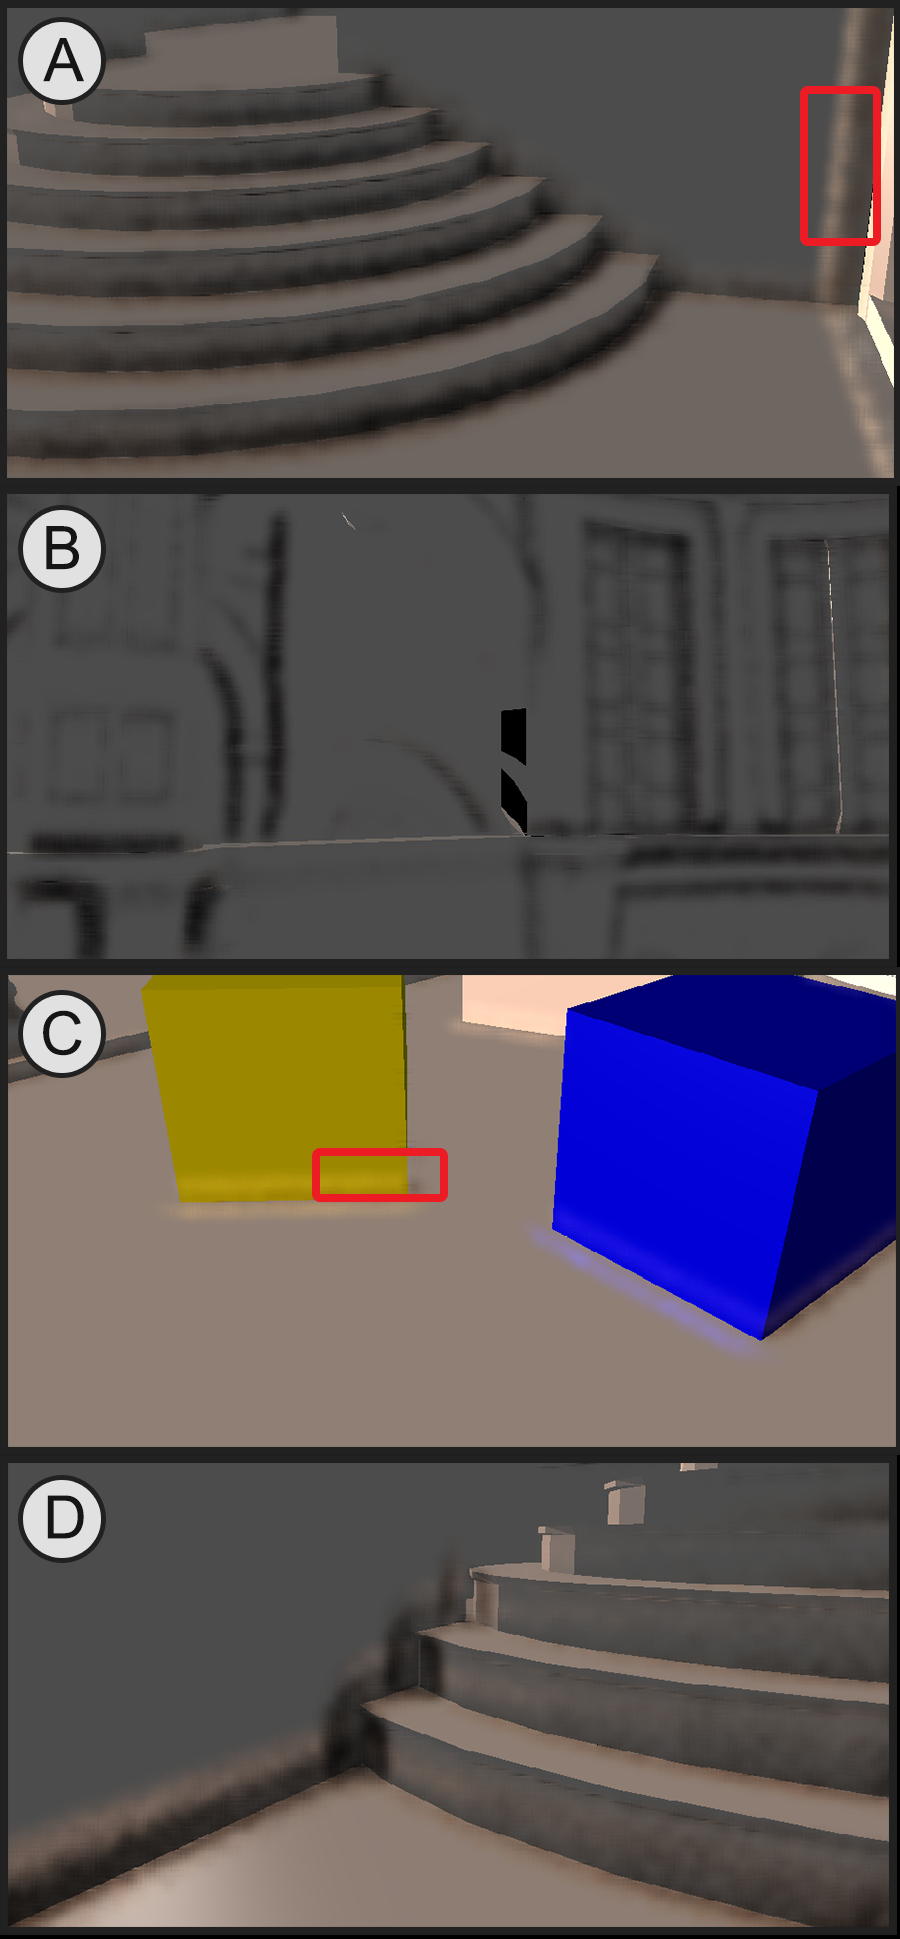
\includegraphics[width=0.3\textwidth]{fig_4_A.png}
		\caption{Visual results of SSDO-A technique.}
		\label{fig:4_A}
	\end{figure}

	\pagebreak

	\begin{figure}[ht]
		\centering
		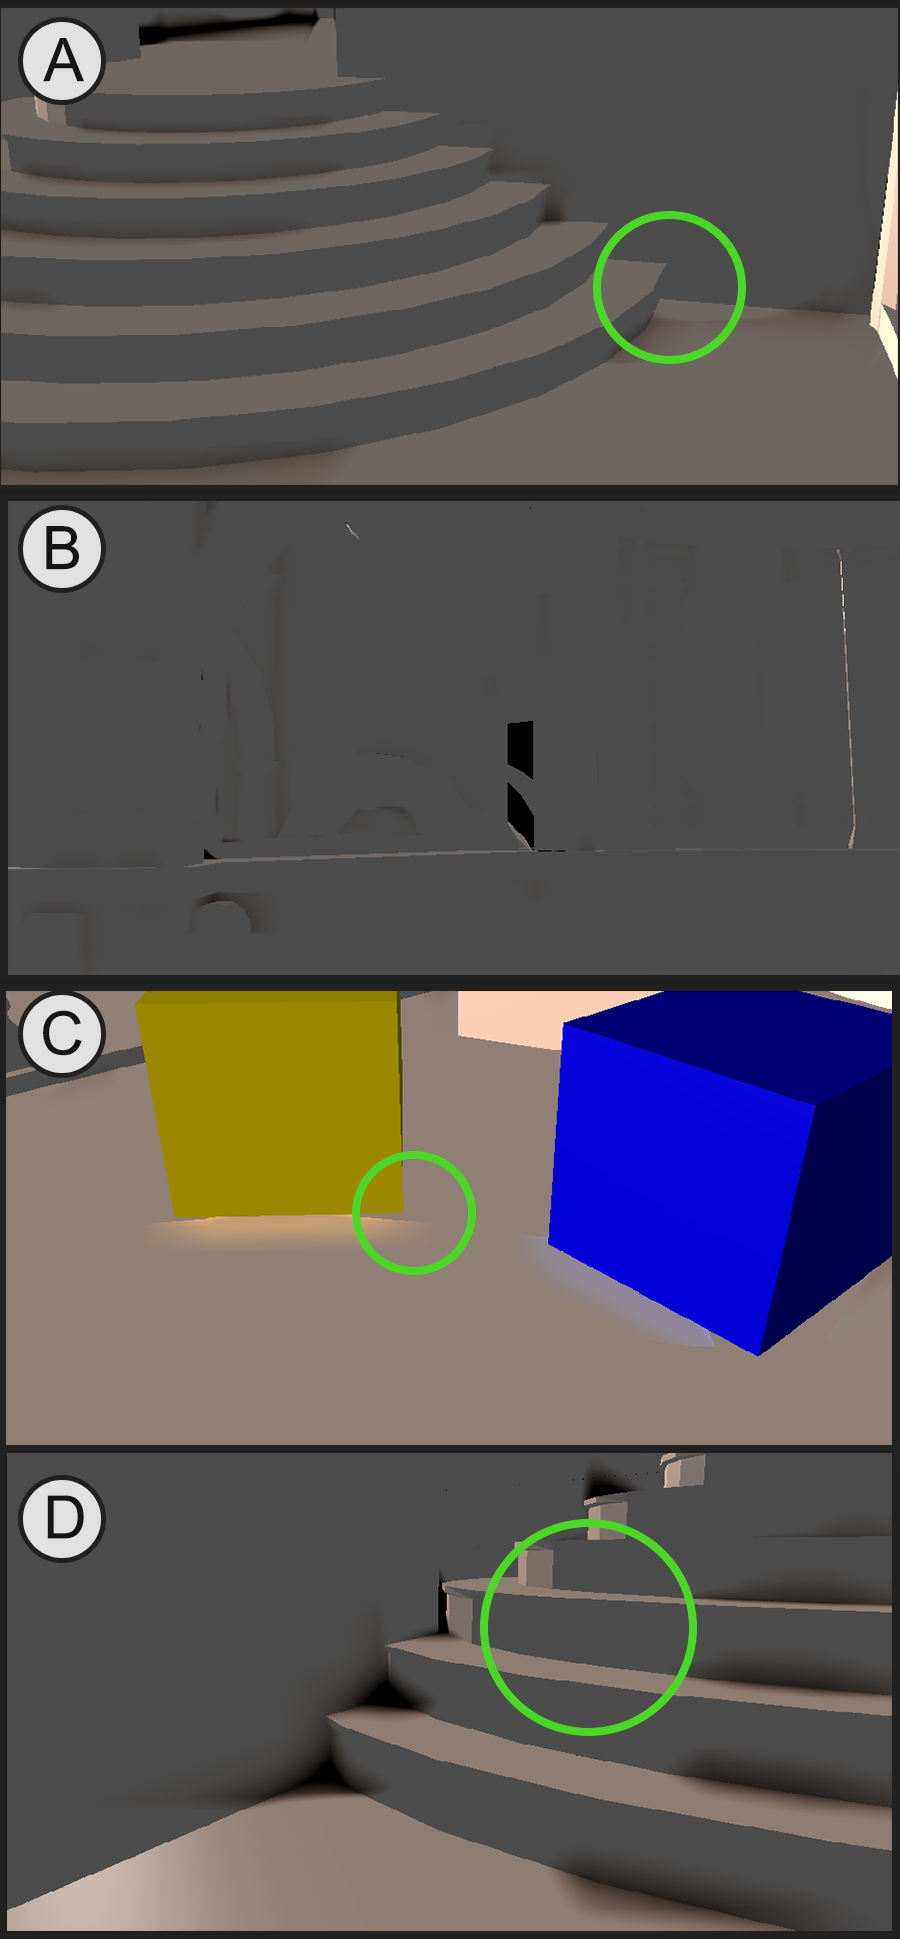
\includegraphics[width=0.3\textwidth]{fig_4_B.png}
		\caption{Visual results of SSDO-B technique.}
		\label{fig:4_B}
	\end{figure}

	\begin{figure}[ht]
		\centering
		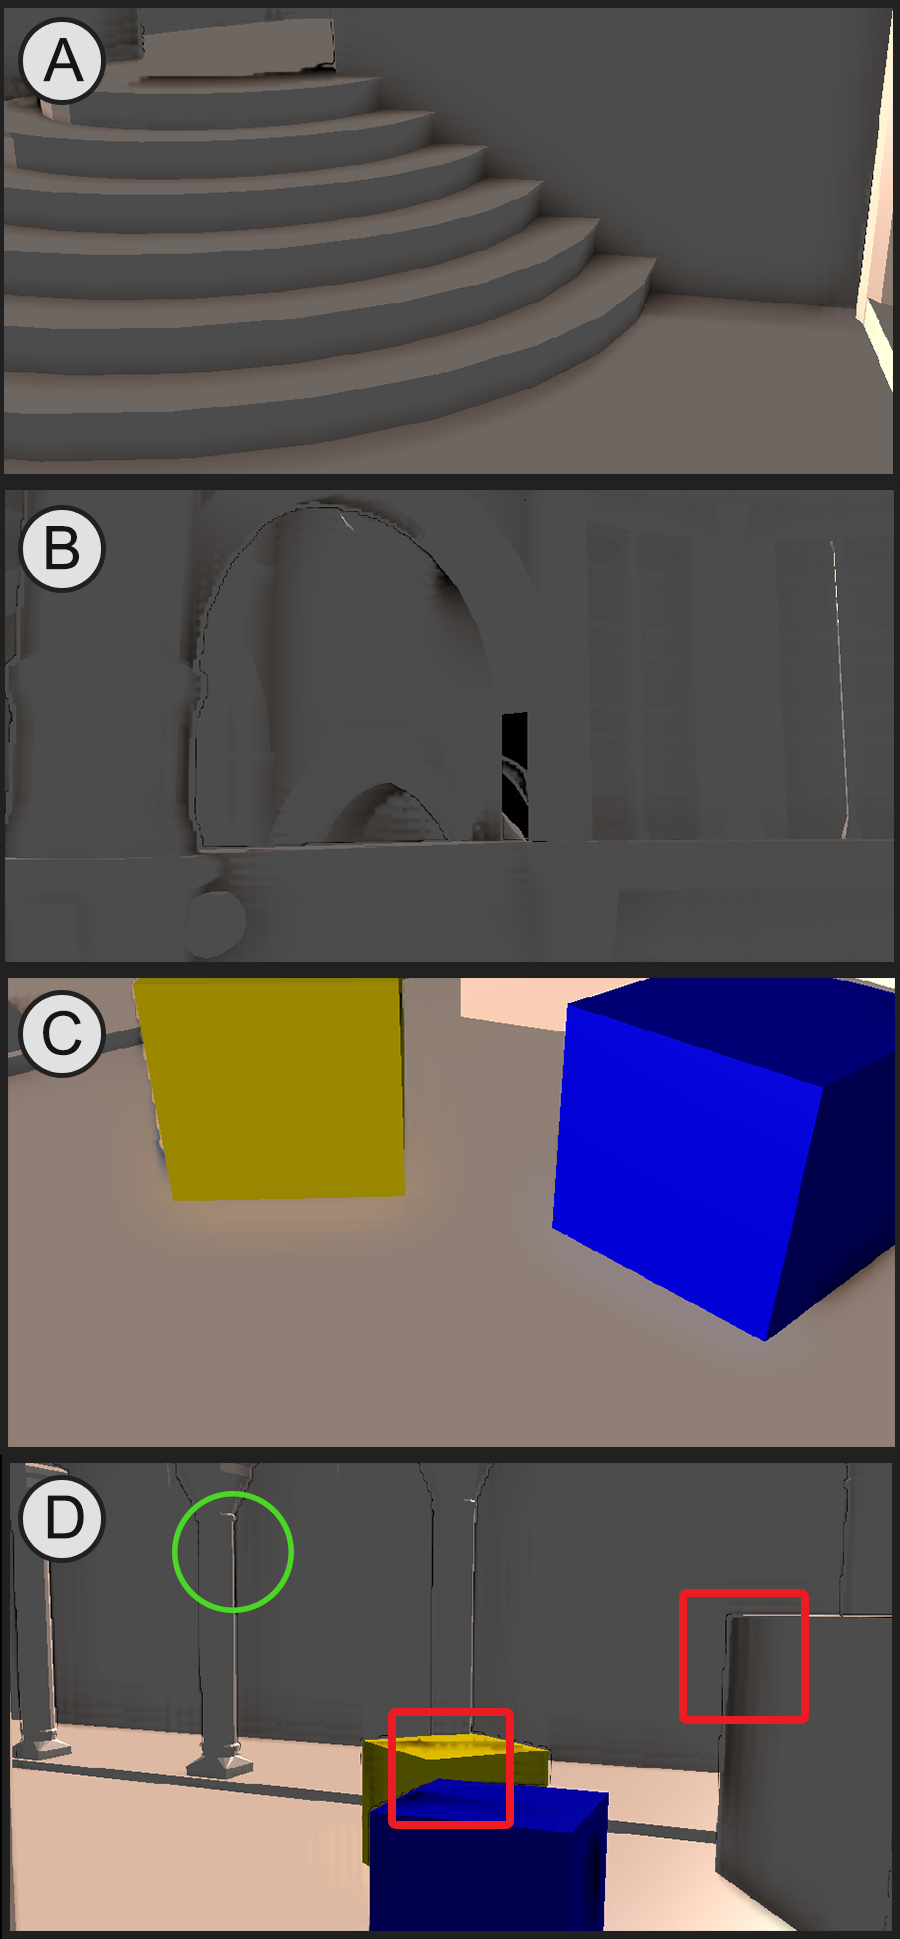
\includegraphics[width=0.3\textwidth]{fig_4_C.png}
		\caption{Visual results of SSDO-C technique.}
		\label{fig:4_C}
	\end{figure}

	\pagebreak

\section{Conclusion}\label{t:conclusion}

Despite previous assumptions, SSDO-B performed two times slower than its archetype and almost six times than SSDO-A. Letting a 16.67 ms be a maximum time an one frame can be rendered in (equals 60 FPS), this method needs 2.41 ms for computation which is 14\% of total time. It is a very high value and expels the technique from any practical employment. In spite of using statistical model, which requires much less samples for one pixel, no performance gain was obtained. The reason for this is the adaptive layer technique. Creating SAT only for main buffers would not have such a great impact, but aforementioned method requires this computation done five times in one frame. Because of the fact that SSDO requires averaged colour buffer as well, data set is twice as big than in original StatVO implementation. These two factors are main reason of this serious performance drop. In one frame, thirteen compute shader Dispatch calls and six shader changes take place. This is hardly avoidable because of the necessity to keep the proper order of operations.

The situation is much better in case of the SSDO-C method. On the figure \ref{wykr_7_A} it can easily be seen that this is the fastest technique. Computations take only 0.12 ms which is 0.7\% of the assumed total frame time. Their speed is 2.5 times higher than speed of the SSDO-A. The reason of this performance boost is removal of whole SAT and adaptive layer generation. They were replaced with simple depth-aware Gaussian blur of the second mip level of base textures. In result, the amount of computations and number of Dispatch calls was drastically lowered. Only two passes of blurring are performed in one frame -- vertical and horizontal. Third pass is the main pass of the SSDO-C technique. Sampling process is simplified comparing to the SSDO-B as well, because it requires obtaining only one sample per buffer, instead of four. Neither averages nor differences between values are computed as well.

Out of the two implemented techniques, SSDO-B generates more visible errors and artifacts. It was presented on pictures A, C and D of figure \ref{fig:4_B} and marked with green circles. It is visible that in these places a hard border between darkened and non-darkened occur. A reason for that is the usage of adaptive layer system. Non-assigned pixels on each layer are filled with zeroes. During the computation of an average value, these zeroes have influence on the final value. It results in ``holes'' in occlusion effect. In places where it is visible, as well as in SSDO-C, it can be noticed that the result differs from the one produced by SSDO-A. Because the statistical model was used, no noise appears and the effect is very smooth but also much more subtle (screenshots A and B of figure \ref{fig:4_C} and figure \ref{fig:4_A}). The same properties apply to indirect lighting. What needs to be mentioned is that a reflection from the floor does not occur in SSDO-B and SSDO-C methods (marked with red rectangles on figure \ref{fig:4_A}). Whether it is an improvement or an error is a completely subjective matter. One of the greatest limitations of this technique is the number of layers. For more complex scenes it may not be enough to prevent dark halos around objects from appearing. Further multiplication of the layer count will result in even greater performance drop. Also it needs to be mentioned that SAT generation algorithm needs to use a continuous shared memory block per texture row. This limits maximum buffer size to twice the maximum thread count in a compute shader thread group, which results in 2048 on Direct3D 11. Texture can be split into parts which are computed separately and then combined, but this will result in a serious performance drop.

The SSDO-C technique is free of holes in darkening because it does not use adaptive layering. On the pictures B~and D of figure \ref{fig:4_C} aforementioned dark edge border artifact can be seen (marked with green circle), which is a result of an edgy depth buffer. A method proposed to solve this issue is not completely effective and its results depend on the distance from the camera. A second issue is ``occlusion bleeding'' on flat surfaces near the depth discontinuities. A reason of this is distortion generated by simple but efficient blurring algorithm. It can be seen only from specific directions of the camera. The last important issue is that ``directness'' of the occlusion is much less visible than in SSDO-A, what can be easily noticed by comparing left side of pictures A of figures \ref{fig:4_C} and \ref{fig:4_A}. After solving these three issues, SSDO-C could be successfully used in practice, for example in game engine, as an efficient and noise-free directional occlusion generating algorithm.

	\subsection{Future work}\label{t:conclusion:futurework}
	
	To use SSDO-B technique in practice a SAT and adaptive layer generation process need to be simplified. Also, a layer discontinuity has to be solved. First issue could be repaired by combining all computation into one global compute shader, but inability to synchronize code execution between thread groups makes this a non-trivial concept.
	
	To improve upon SSDO-C technique one should employ more complex depth-aware blurring algorithms, to eliminate edge issues and remove ``occlusion bleeding''. In the first matter using a hybrid method may help, i.e. introducing limited amount of sampling in the neighbourhood of the pixel to detect edges more successfully. Employing an efficient anti-aliasing algorithm could also be a promising direction. To make the directional factor be more visible, as it is in SSDO-A, one could use varying size of blur kernel, depending on an angle between normal vector and light direction.

%\section*{Acknowledgment}
% The authors would like to thank...

\begin{thebibliography}{99}
\bibitem{ao} S. Zhukov, A. Iones, G. Kronin, \emph{An Ambient Light Illumination Model}, Eurographics Rendering Workshop, 1998

\bibitem{statvo} Quintjin Hendrickx, Leonardo Scandolo, Martin Eisemann, Elmar Eisemann, \emph{Adaptively Layered Statistical Volumetric Obscurance}, High Performance Graphics, 2015

\bibitem{ssdo} Tobias Ritschel, Thorsten Grosch, Hans-Peter Seidel, \emph{Approximating Dynamic Global Illumination in Image Space}, Association for Computing Machinery, Inc., 2009

\bibitem{sloan} B. Loos, J. Sloan, \emph{Volumetric obscurance}, ACM SIGGRAPH, 2010

\bibitem{sat} Marcos Slomp, Toru Tamaki, Kazufumi Kaneda, emph {Screen-Space Ambient Occlusion Through Summed-Area Tables}, First International Conference on Networking and Computing, 2010

\bibitem{prefix-sum} Mark Harris, \emph{Parallel Prefix Sum (Scan) with CUDA}, Nvidia, 2007

\bibitem{directcompute} Eric Young, \emph{DirectCompute Optimizations and Best Practices}, Nvidia, GPU Technology Conference, 2010

\bibitem{crytek} M. Mittring, \emph{Finding next gen: Cryengine 2}, ACM SIGGRAPH, 2007

\end{thebibliography}

\begin{IEEEbiography}{Dominik Szajerman}
Biography text here.
\end{IEEEbiography}

\begin{IEEEbiography}[{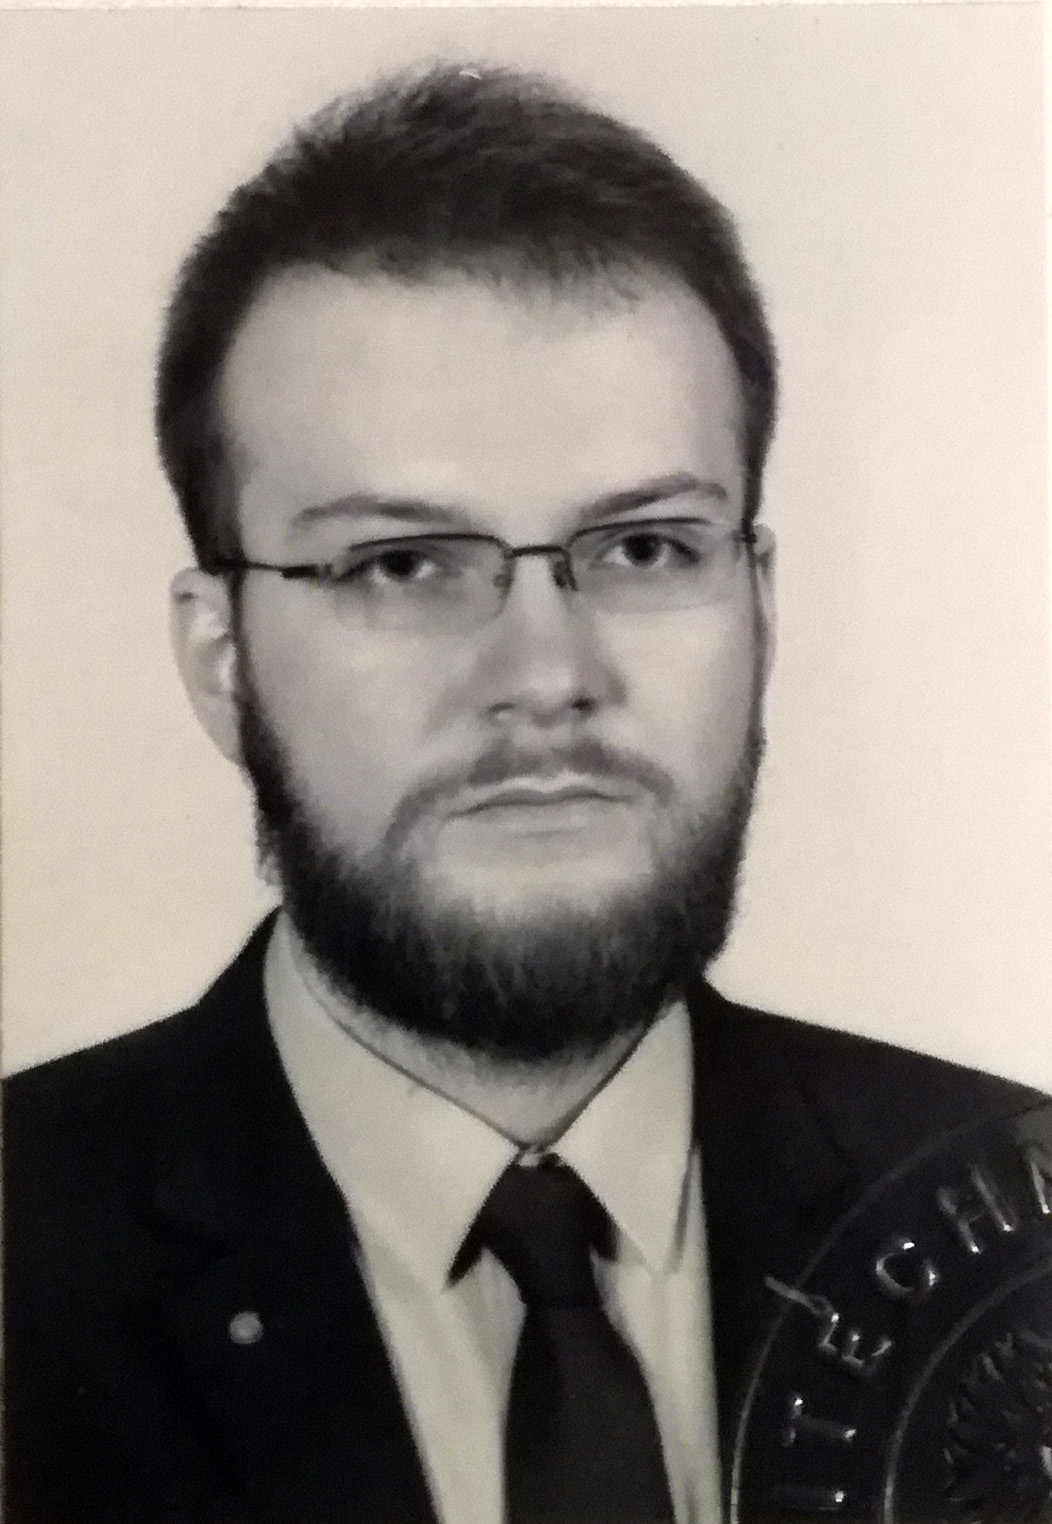
\includegraphics[width=1in,height=1.25in,clip,keepaspectratio]{focia.jpg}}]
{Marcin Wawrzonowski}
BSc –- a graduate of the first degree studies in Information Technology at the Faculty of Technical Physics, Information Technology and Applied Mathematics at Lodz University of Technology in specialization Computer Simulation and Games Technology – thesis topic: ``A physical cloth simulation using GPU of mobile devices''. Participant of EU project ``Informatyka -- kierunek zamawiany na Politechnice {\L}{\'o}dzkiej'' in the ``Computer Graphics in Entertainment and Computer Games'' module. Co-creator of published Android game ``Rocket Thruster'' developed within the this project.
\end{IEEEbiography}

\enlargethispage{-5in}

\end{document}


